\section{Method}
\label{sec:hybrid-approach}
\paragraph{Method Overview}

\hybrid{} consists of a \textsc{Constructor} $\mathcal{F}_c$, a \textsc{Weighter} $\mathcal{F}_w$, and a \textsc{LinearHead} $\mathcal{F}_l$. At a high level, the \textsc{Constructor} $\mathcal{F}_c$ is responsible for identifying hyperedges $H$ from the data to construct the hypergraph. After that, the \textsc{Weighter} $\mathcal{F}_w$ calculates a weight for each hyperedge. Finally, based on all the weights $\boldsymbol{w}$, the \textsc{LinearHead} $\mathcal{F}_l$ predicts the label $Y$.
An illustration of this pipeline is shown in Figure \ref{fig:pipeline}. The pipeline can be formulated as
\begin{equation}
% \vspace{-1em}
    \label{equ:pipeline}
    X \xrightarrow[\mathcal{F}_c]{} H \xrightarrow[\mathcal{F}_w]{} \boldsymbol{w}\xrightarrow[\mathcal{F}_l]{} Y.
\end{equation}

We will elaborate on the details of the architecture below.

\begin{figure*}
\vspace{0.8em}
    \centering
    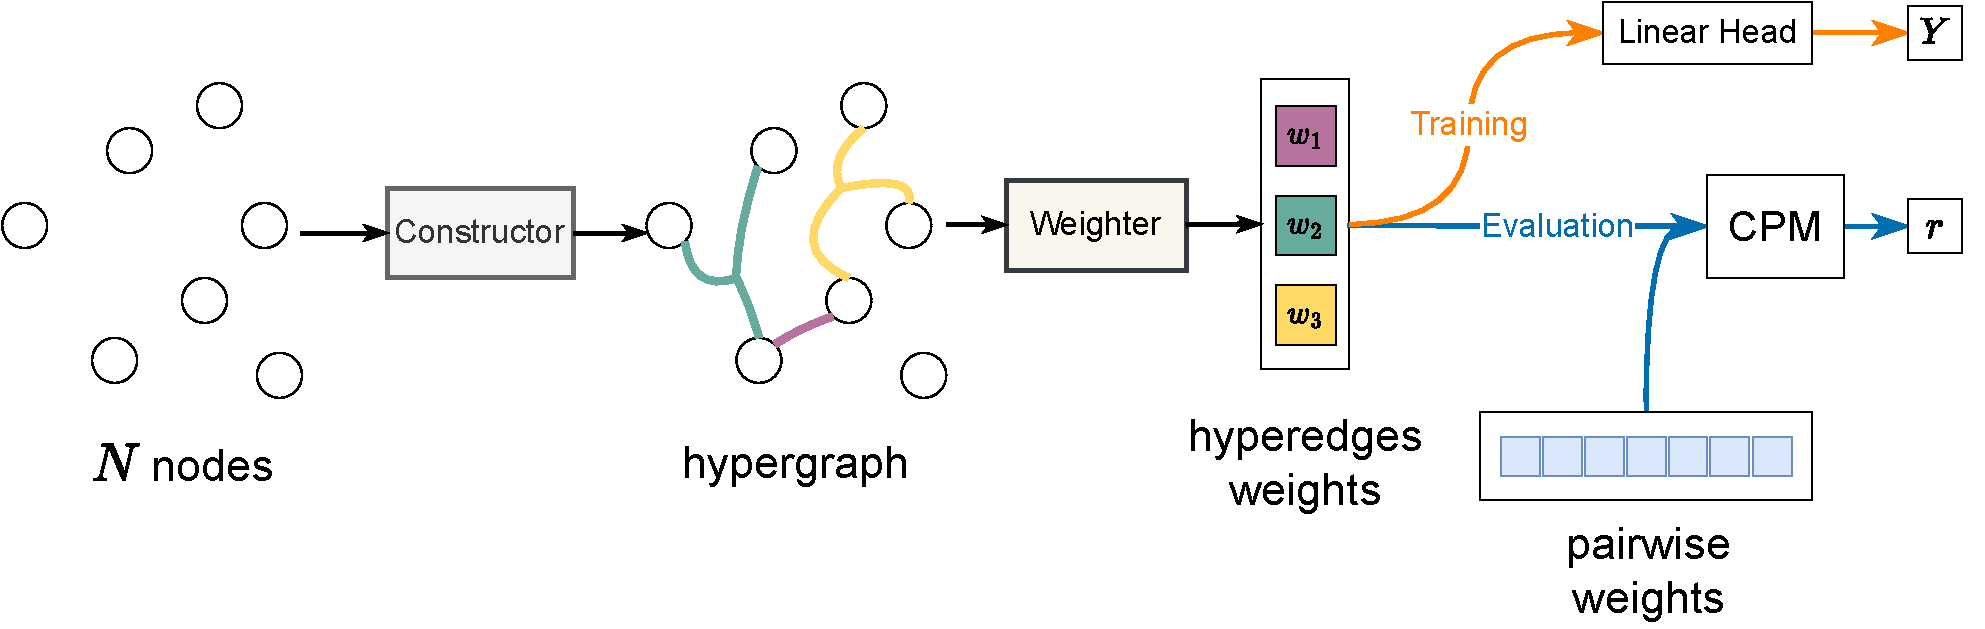
\includegraphics[width=\linewidth]{figures/pipeline2.drawio.pdf}
    % \vskip 0.1in
    \caption{Overview of the \hybrid{} pipeline when the total number of hyperedges $K=3$. Hyperedge are in distinct colors for clarity.  The \textsc{Constructor} identifies hyperedges in the hypergraph, where regions are nodes. The \textsc{Weighter} computes a weight for each hyperedge. These weights, representing strengths of hyperedges, are expected to be informative in terms of our target $Y$. There are two separate phases after obtaining weights of hyperedges: 1) Training. The model's parameters are trained under the supervision of $Y$; 2) Evaluation. The output weights, as well as pairwise weights, are fed into the CPM \citep{shen2017using}.}
    \label{fig:pipeline}
    % \vskip -0.1in
\end{figure*}

\subsection{Learning the Hypergraph by Multi-head Masking}
\label{sec:learn-by-mask}

Each instance (human subject) is represented by $X = [X_1, X_2, \cdots, X_N]^T \in \mathbb{R}^{N\times d}$, where $X_i \in \mathbb{R}^d$ is a column vector representing the features of region $i$. These regions are nodes in the hypergraph we are going to construct. Hyperedges in the hypergraph can be beneficial in the learning process below because it is essential to model the relationships between more than two regions.

\paragraph{Hyperedges Construction}
In this paragraph, we elaborate on how the \textsc{Constructor} identifies the hyperedges, i.e. $H=\mathcal{F}_c(X)$.

Suppose the number of hyperedges is $K$, which is a predefined hyperparameter. We assign a head to each hyperedge. Each head is responsible for constructing a hyperedge by selecting nodes belonging to that hyperedge. 

Specifically, to construct the $k$-th hyperedge, the \textsc{Constructor}'s $k$-th head outputs a column vector $\boldsymbol{m}^k \in \{0,1\}^N$, where each element in the vector corresponds to a brain region,

\begin{equation}
\label{equ:shallow}
% \begin{aligned}
\boldsymbol{m}^k = [\mathbbm{1}(p^k_{\theta,1}), \mathbbm{1}(p^k_{\theta,2}), \cdots, \mathbbm{1}(p^k_{\theta,N})]^T \in \{0, 1\}^N,
% \end{aligned}
\end{equation}
where $p^k_{\theta, i} \in [0,1], i=1,2,\cdots, N$ are learnable probabilities. $\mathbbm{1}: [0,1] \mapsto \{0,1\} $ is an indicator function, which is defined as $\mathbbm{1}(x) = 1$ if $x > 0.5$ and $\mathbbm{1}(x) = 0$ if $x \leq 0.5$.  And $\boldsymbol{m}^k$ is a column vector corresponding to the $k$-th hyperedge. Note that since there is no gradient defined for the indicator operation, we employ the stop-gradient technique \citep{oord2017neural,bengio2013estimating} to approximate it.

\begin{figure}[t]
    \centering
    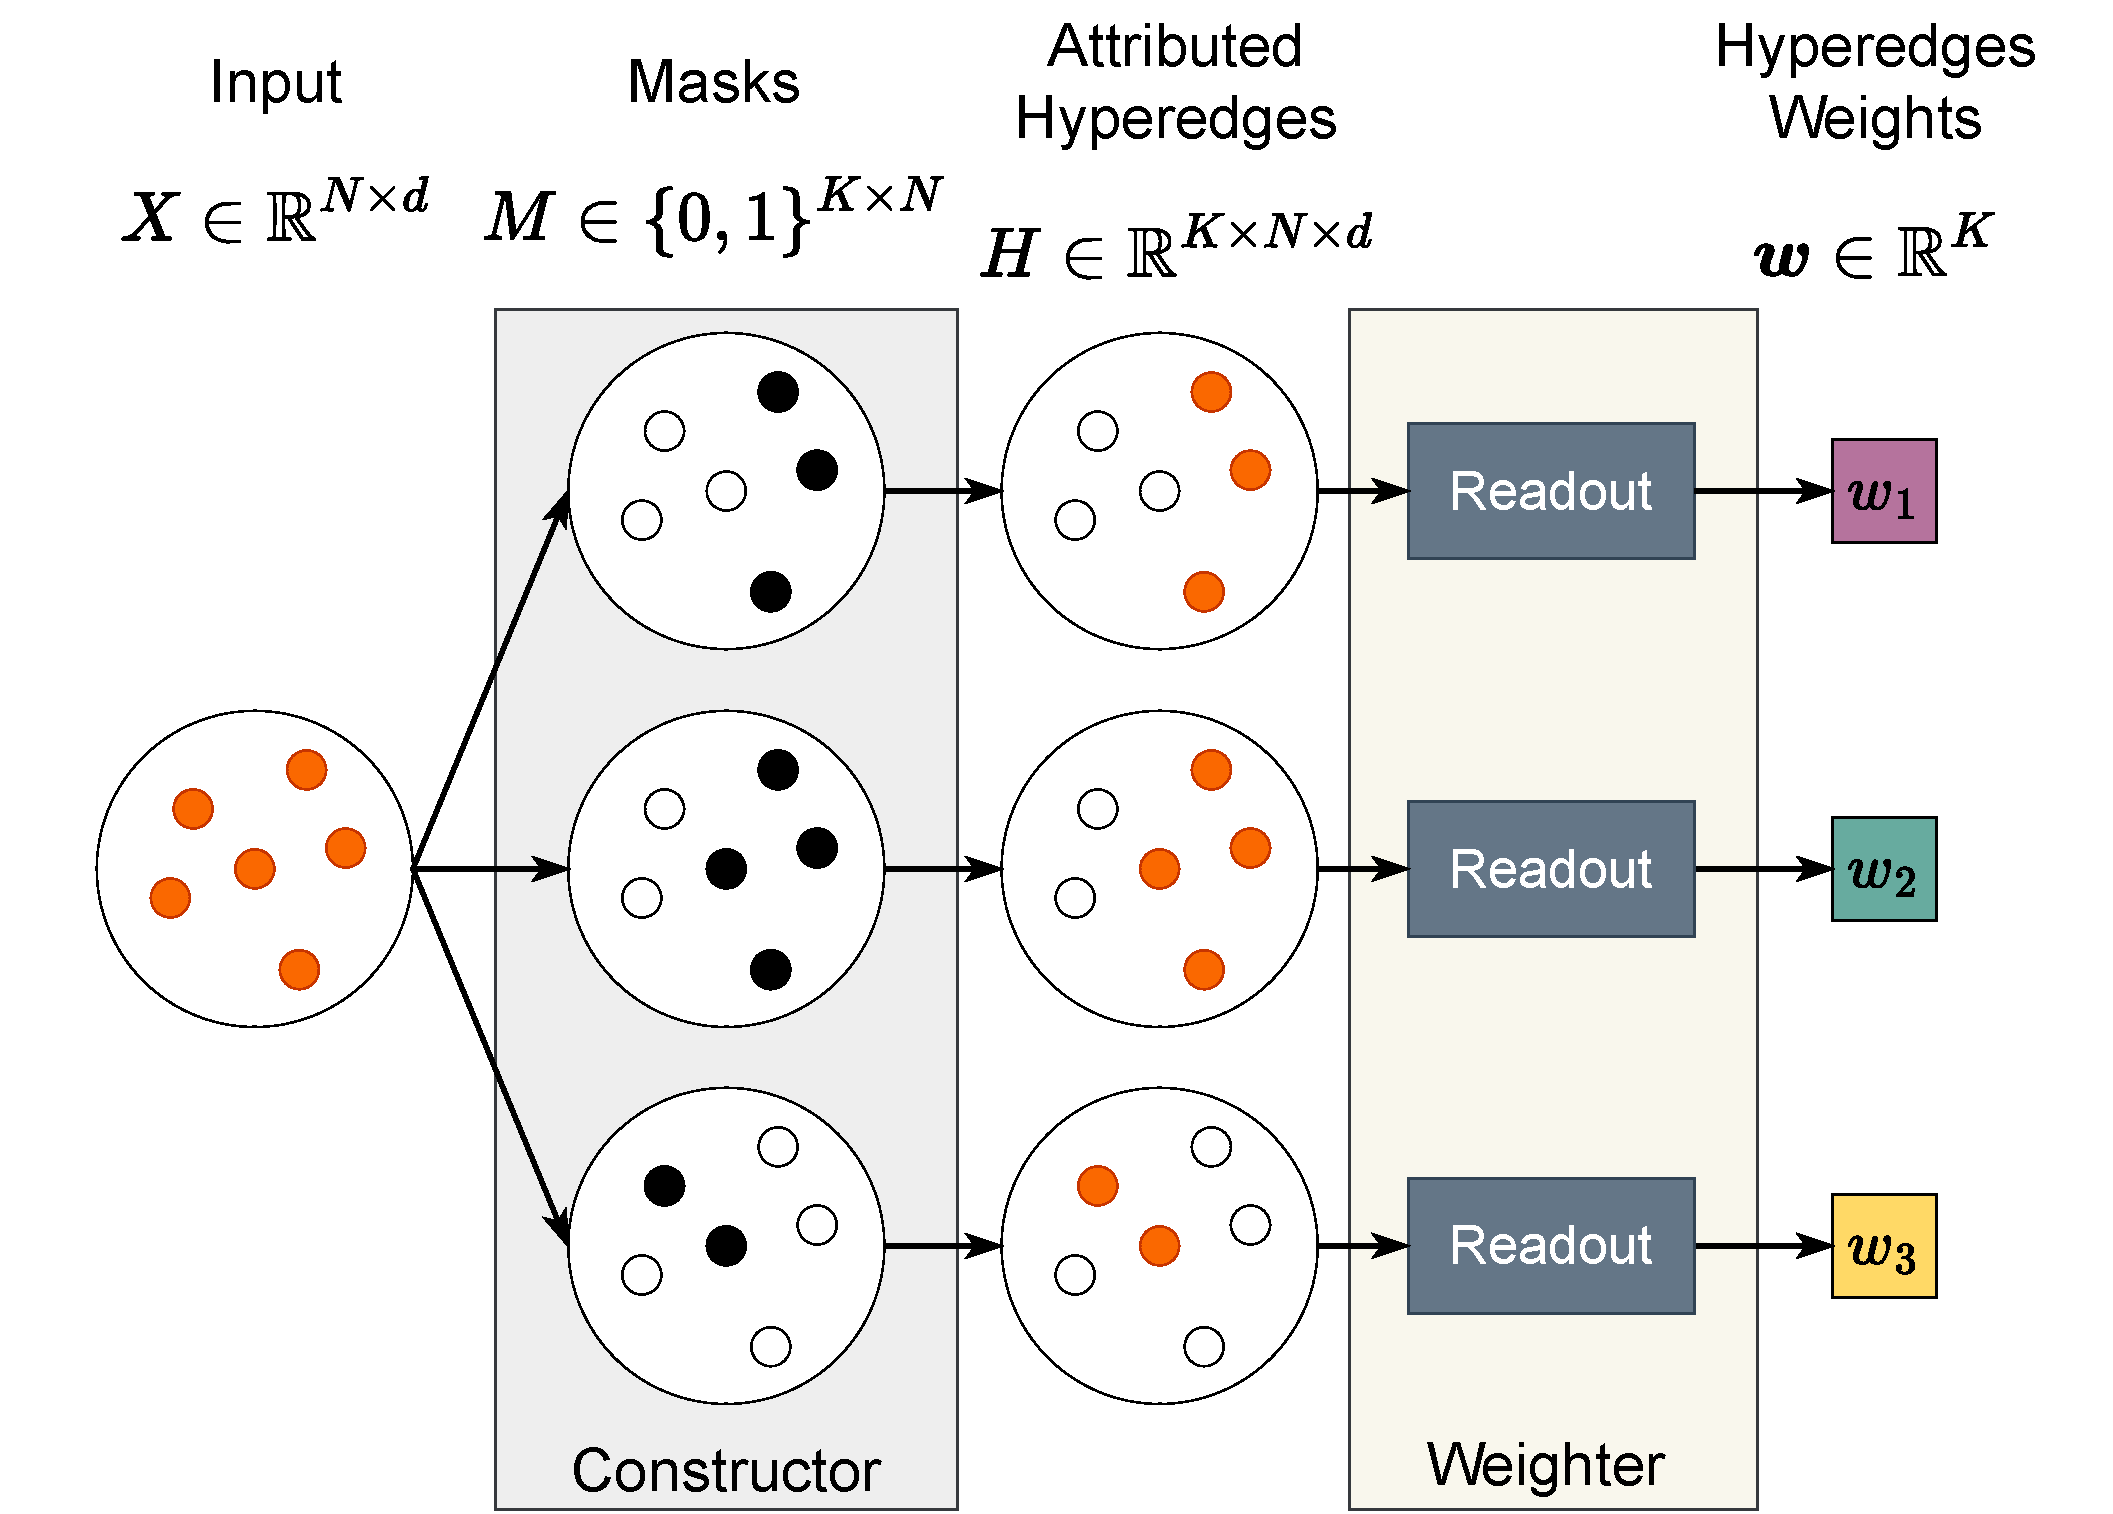
\includegraphics[width=0.63\linewidth]{figures/architecture.drawio.pdf}
    \caption{Architecture details of the \textsc{Constructor} and the \textsc{Weighter}  when the number of nodes $N=6$ and the number of hyperedges $K=3$. At a high level, the \textsc{Constructor} learns the hyperedge structure by masking nodes. The \textsc{Weighter} computes the weight of each hyperedge based on the hyperedge's member nodes and their features.}
    \label{fig:enter-label}
\end{figure}

In the vector $\boldsymbol{m}^k$, $0$ indicates nodes that are masked out, and $1$ indicates nodes that are not masked. Nodes that are not masked are considered to form a hyperedge together. We use $\boldsymbol{h}^k$ to represent the masked version of $X$
\begin{equation}
\begin{aligned}
    \boldsymbol{h}^k &= \boldsymbol{m}^k \odot X \\&= [\boldsymbol{m}^k_1 X_1, \boldsymbol{m}^k_2 X_2, \cdots, \boldsymbol{m}^k_N X_N] \in \mathbb{R}^{N\times d},   
\end{aligned}
\end{equation}
where $\odot$ is the broadcast element-wise multiplication. $\boldsymbol{m}^k_j$ is the $j$-th element of the vector $\boldsymbol{m}^k$.  

We obtain $K$ hyperedges for $K$ sets of masks. We use $H$ to denote the collection of all hyperedges.
\begin{equation}
    H = (\boldsymbol{h}^1, \boldsymbol{h}^2, \cdots, \boldsymbol{h}^K).
\end{equation} 

\paragraph{Hyperedge Weighting}
After obtaining the structure (i.e. member nodes) of each hyperedge,  the \textsc{Weighter} will calculate each hyperedge's weight, which is supposed to indicate the importance of that hyperedge, based on the member nodes and their features, i.e. $\boldsymbol{w} = \mathcal{F}_w(H)$.

These weights are obtained by a $\operatorname{Readout}$ module, which is composed of: 1) summing over all the non-masked nodes feature-wisely; 2) dim reduction operation.

\begin{equation}
\label{equ:readout}
    w^k = \operatorname{Readout}(\boldsymbol{h}^k) = \operatorname{DimReduction}({\boldsymbol{m}^k}^T\boldsymbol{h}^k) \in \mathbb{R},
\end{equation}

where $w^k$ is the weight of the $k$-th hyperedge and $\operatorname{DimReduction}$ is an MLP with ReLU activations, where the output dimension is $1$.
For all hyperedges, we obtain $K$ hyperedges in total, $\boldsymbol{w} = [w^1, w^2, \cdots, w^K]^T \in \mathbb{R}^K$. Finally, these weights will be fed into the final linear head to predict the label of the instance, 
\begin{equation}
\label{equ:linearhead}
    \hat{Y} = \mathcal{F}_l(\boldsymbol{w}) \in \mathbb{R}.
\end{equation}

In contrast to previous hypergraph construction methods \citep{jin2019robust,xiao2019multi}, which identify hyperedges by refining neighbors and simply aggregating node features, \hybrid{} makes these procedures learnable and thus is able to identify MIMR hyperedges in a data-driven way through expressive neural networks. The Full study that decides the number of hyperedges $K$ is provided in \cite{qiu2023learning}.

\paragraph{Computational Complexity}
The computational complexity of our model is $O(N^2K)$, which is just the same scale as that of MLPs even though we are addressing a more challenging task: identifying high-order relationships in an exponential space. Details of the complexity calculation can be found in \cite{qiu2023learning}


\subsection{Optimization Framework}
 Since there are no existing IB frameworks that can be applied in our context, we propose a new IB framework named \multiheadname{} to optimize \hybrid{}. To adopt an information bottleneck view of \hybrid{}, we consider $X$, $Y$ and $H$ are random variables in the Markovian chain $X \leftrightarrow Y \leftrightarrow H$. According to our MIMR objective, we optimize
\begin{equation}
\label{equ:ib2}
    \arg \max I(H; Y) - \beta I(H; X),
\end{equation}
where $I(\cdot ; \cdot)$ denotes the mutual information. $I(H; Y)$ corresponds to the informativeness and $I(H; X)$ corresponds to the redundancy. $\beta$ is a coefficient trading off informativeness and redundancy. Since optimizing the mutual information for high-dimensional continuous variables is intractable, we instead optimize the lower bound of Equation \ref{equ:ib2}. Specifically, for the first term (informativeness), it is easy to show
\begin{equation}
\label{equ:lowerbound}
\begin{aligned}
    I(H; Y) &= \mathbb{H}[Y] -  \mathbb{H}[{Y|H}] \\
    &=\mathbb{H}[Y] + \mathbb{E}_{p(Y, H)}[\log p(Y|H)] \\
    & = \mathbb{H}[Y] + \mathbb{E}_{p(Y, H)}[\log q_\phi(Y|H)] \\
    &\quad + \mathbb{E}_{p(H)}[\operatorname{KL}(p(Y|H)|q_\phi(Y|H))] \\
   & \geq \mathbb{H}[Y] + \mathbb{E}_{p(Y, H)}[\log q_\phi(Y|H)],
\end{aligned}
\end{equation}
where $\mathbb{H}[\cdot]$ is the entropy computation.
Since there is no learnable component in the entropy of $Y$, we only need to optimize the second term $\mathbb{E}_{p(Y, H)}[\log q_\phi(Y|H)]$. $q_\phi$ can be considered as a model that predicts $Y$ based on $H$, which essentially corresponds to $\mathcal{F}_l \circ \mathcal{F}_w$, where $\circ$ is the function composition. In practice, we set $q_\phi$ as a Gaussian model with variance $1$ as most probabilistic machine learning models do for continuous data modeling \citep{alemi2016deep,luo2019significance,peng2018variational,kingma2013auto}. 


For the second term (redundancy) in Equation \ref{equ:ib2}, we have

\begin{proposition}
    (Upper bound of $I(H;X)$ in \multiheadname{})
\begin{equation}
\label{equ:multi_drop}
    \begin{aligned}
        I(H; X) 
        \leq \sum_{k=1}^K
        I(\boldsymbol{h}^k; X)
        &\leq \sum_{k=1}^K \sum_{i=1}^N
        I(\boldsymbol{h}^k_i; X_i)\\
        &= \sum_{k=1}^K\sum_{i=1}^N \mathbb{H}[X_i] (1 - p^k_{\theta, i}),
    \end{aligned}
\end{equation}
\end{proposition}

where $\boldsymbol{h}^k_i$ and $X_i$  is the $i$-th row of $\boldsymbol{h}^k$ and $X$ respectively.  $p^k_{\theta,i}$ is the mask probability in Equation \ref{equ:shallow}. $\mathbb{H}$ is the entropy computation. The equality holds if and only if nodes are independent and hyperedges do not overlap. It's important to clarify that optimizing Equation \ref{equ:multi_drop} does not imply a penalty for overlaps. The second inequality is inspired by \cite{kim2021drop}. The proof of the proposition can be found in \citet{qiu2023learning}.


% \begin{equation}
%     \mathcal{F}_c(X) =  \mathbbm{1}(p_\theta) \odot X
% \end{equation}
% \begin{equation}
%     q_\phi (H) =\mathcal{F}_l \circ \mathcal{F}_w (H)
% \end{equation}
Therefore, instead of optimizing the intractable objective Equations \ref{equ:ib2}, we optimize its upper bound (i.e. loss function) according to Equations \ref{equ:lowerbound} and \ref{equ:multi_drop}.
\begin{equation}
\begin{aligned}
    \mathcal{L} &= \| Y - \mathcal{F}_l \circ \mathcal{F}_w \circ \mathcal{F}_c (X) \|_2^2 + \beta \sum_{k=1}^K\sum_{i=1}^N \mathbb{H}[X_i] (1 - p^k_{\theta,i}) \\&\geq - I(H, Y) + \beta I(H, X).
\end{aligned}
\end{equation}
In conclusion, The learnable components are the shallow embeddings in Equation \ref{equ:shallow}, the $\operatorname{DimReduction}$ MLP in Equation \ref{equ:readout} and the \textsc{LinearHead} $\mathcal{F}_l$ in Equation \ref{equ:linearhead}.